% Options for packages loaded elsewhere
\PassOptionsToPackage{unicode}{hyperref}
\PassOptionsToPackage{hyphens}{url}
%
\documentclass[
  ignorenonframetext,
]{beamer}
\usepackage{pgfpages}
\setbeamertemplate{caption}[numbered]
\setbeamertemplate{caption label separator}{: }
\setbeamercolor{caption name}{fg=normal text.fg}
\beamertemplatenavigationsymbolsempty
% Prevent slide breaks in the middle of a paragraph
\widowpenalties 1 10000
\raggedbottom
\setbeamertemplate{part page}{
  \centering
  \begin{beamercolorbox}[sep=16pt,center]{part title}
    \usebeamerfont{part title}\insertpart\par
  \end{beamercolorbox}
}
\setbeamertemplate{section page}{
  \centering
  \begin{beamercolorbox}[sep=12pt,center]{part title}
    \usebeamerfont{section title}\insertsection\par
  \end{beamercolorbox}
}
\setbeamertemplate{subsection page}{
  \centering
  \begin{beamercolorbox}[sep=8pt,center]{part title}
    \usebeamerfont{subsection title}\insertsubsection\par
  \end{beamercolorbox}
}
\AtBeginPart{
  \frame{\partpage}
}
\AtBeginSection{
  \ifbibliography
  \else
    \frame{\sectionpage}
  \fi
}
\AtBeginSubsection{
  \frame{\subsectionpage}
}
\usepackage{amsmath,amssymb}
\usepackage{iftex}
\ifPDFTeX
  \usepackage[T1]{fontenc}
  \usepackage[utf8]{inputenc}
  \usepackage{textcomp} % provide euro and other symbols
\else % if luatex or xetex
  \usepackage{unicode-math} % this also loads fontspec
  \defaultfontfeatures{Scale=MatchLowercase}
  \defaultfontfeatures[\rmfamily]{Ligatures=TeX,Scale=1}
\fi
\usepackage{lmodern}
\ifPDFTeX\else
  % xetex/luatex font selection
\fi
% Use upquote if available, for straight quotes in verbatim environments
\IfFileExists{upquote.sty}{\usepackage{upquote}}{}
\IfFileExists{microtype.sty}{% use microtype if available
  \usepackage[]{microtype}
  \UseMicrotypeSet[protrusion]{basicmath} % disable protrusion for tt fonts
}{}
\makeatletter
\@ifundefined{KOMAClassName}{% if non-KOMA class
  \IfFileExists{parskip.sty}{%
    \usepackage{parskip}
  }{% else
    \setlength{\parindent}{0pt}
    \setlength{\parskip}{6pt plus 2pt minus 1pt}}
}{% if KOMA class
  \KOMAoptions{parskip=half}}
\makeatother
\usepackage{xcolor}
\newif\ifbibliography
\usepackage{graphicx}
\makeatletter
\def\maxwidth{\ifdim\Gin@nat@width>\linewidth\linewidth\else\Gin@nat@width\fi}
\def\maxheight{\ifdim\Gin@nat@height>\textheight\textheight\else\Gin@nat@height\fi}
\makeatother
% Scale images if necessary, so that they will not overflow the page
% margins by default, and it is still possible to overwrite the defaults
% using explicit options in \includegraphics[width, height, ...]{}
\setkeys{Gin}{width=\maxwidth,height=\maxheight,keepaspectratio}
% Set default figure placement to htbp
\makeatletter
\def\fps@figure{htbp}
\makeatother
\setlength{\emergencystretch}{3em} % prevent overfull lines
\providecommand{\tightlist}{%
  \setlength{\itemsep}{0pt}\setlength{\parskip}{0pt}}
\setcounter{secnumdepth}{-\maxdimen} % remove section numbering
\ifLuaTeX
  \usepackage{selnolig}  % disable illegal ligatures
\fi
\IfFileExists{bookmark.sty}{\usepackage{bookmark}}{\usepackage{hyperref}}
\IfFileExists{xurl.sty}{\usepackage{xurl}}{} % add URL line breaks if available
\urlstyle{same}
\hypersetup{
  pdftitle={ADU Presentation},
  hidelinks,
  pdfcreator={LaTeX via pandoc}}

\title{ADU Presentation}
\author{}
\date{\vspace{-2.5em}2024-02-23}

\begin{document}
\frame{\titlepage}

\begin{frame}{Chicago Additional Dwelling Units}
\protect\hypertarget{chicago-additional-dwelling-units}{}
Maggie Lyman \& Max Wagner
\end{frame}

\begin{frame}{What are ADUs?}
\protect\hypertarget{what-are-adus}{}
\begin{itemize}
\tightlist
\item
  Basement or attic apartment conversions (granny flats)
\item
  Coach houses
\end{itemize}

In May 2021, Chicago passed the ADU ordinance to streamline zoning
requirements for ADU conversion projects in 5 zones: North, Northwest,
West, Southwest, South.

The goal of this program is to increase density and provide additional,
affordable and naturally affordable apartments.
\end{frame}

\begin{frame}{Overview of the ADU Ordinance}
\protect\hypertarget{overview-of-the-adu-ordinance}{}
\begin{itemize}
\tightlist
\item
  Streamlines the zoning process: City Council approval is not required
  to build an ADU
\item
  Removes some parking requirements, increasing affordability of units
\item
  Properties with 2 or more ADUs must set each additional ADU at 60\%
  area median income (AMI)
\item
  Additional requirements for ADUs in South, West, and Southwest zones:
  Buildings with one to three units must be owner-occupied, only two ADU
  permits issued per block per year, cannot construct coach houses on
  vacant lots before a principal residence.
\end{itemize}
\end{frame}

\begin{frame}{Our Research Questions}
\protect\hypertarget{our-research-questions}{}
\begin{enumerate}
\tightlist
\item
  Where are ADUs built in the city? Is there a connection between areas
  with high rent and areas with more ADUs constructed?
\item
  Where are ADU applications denied?
\item
  What kinds of ADUs are built?
\item
  What is the public's perception of ADUs?
\end{enumerate}
\end{frame}

\begin{frame}[fragile]{Where are ADUs built?}
\protect\hypertarget{where-are-adus-built}{}
\begin{verbatim}
## Reading layer `geo_export_6356fb24-e715-483f-922e-9fd4badc2b8c' from data source `C:\Users\mlyma\OneDrive\Documents\GitHub\DAP_Final\geo_export_6356fb24-e715-483f-922e-9fd4badc2b8c.shp' 
##   using driver `ESRI Shapefile'
## Simple feature collection with 801 features and 9 fields
## Geometry type: POLYGON
## Dimension:     XY
## Bounding box:  xmin: -87.94025 ymin: 41.64429 xmax: -87.52366 ymax: 42.02392
## Geodetic CRS:  WGS84(DD)
\end{verbatim}

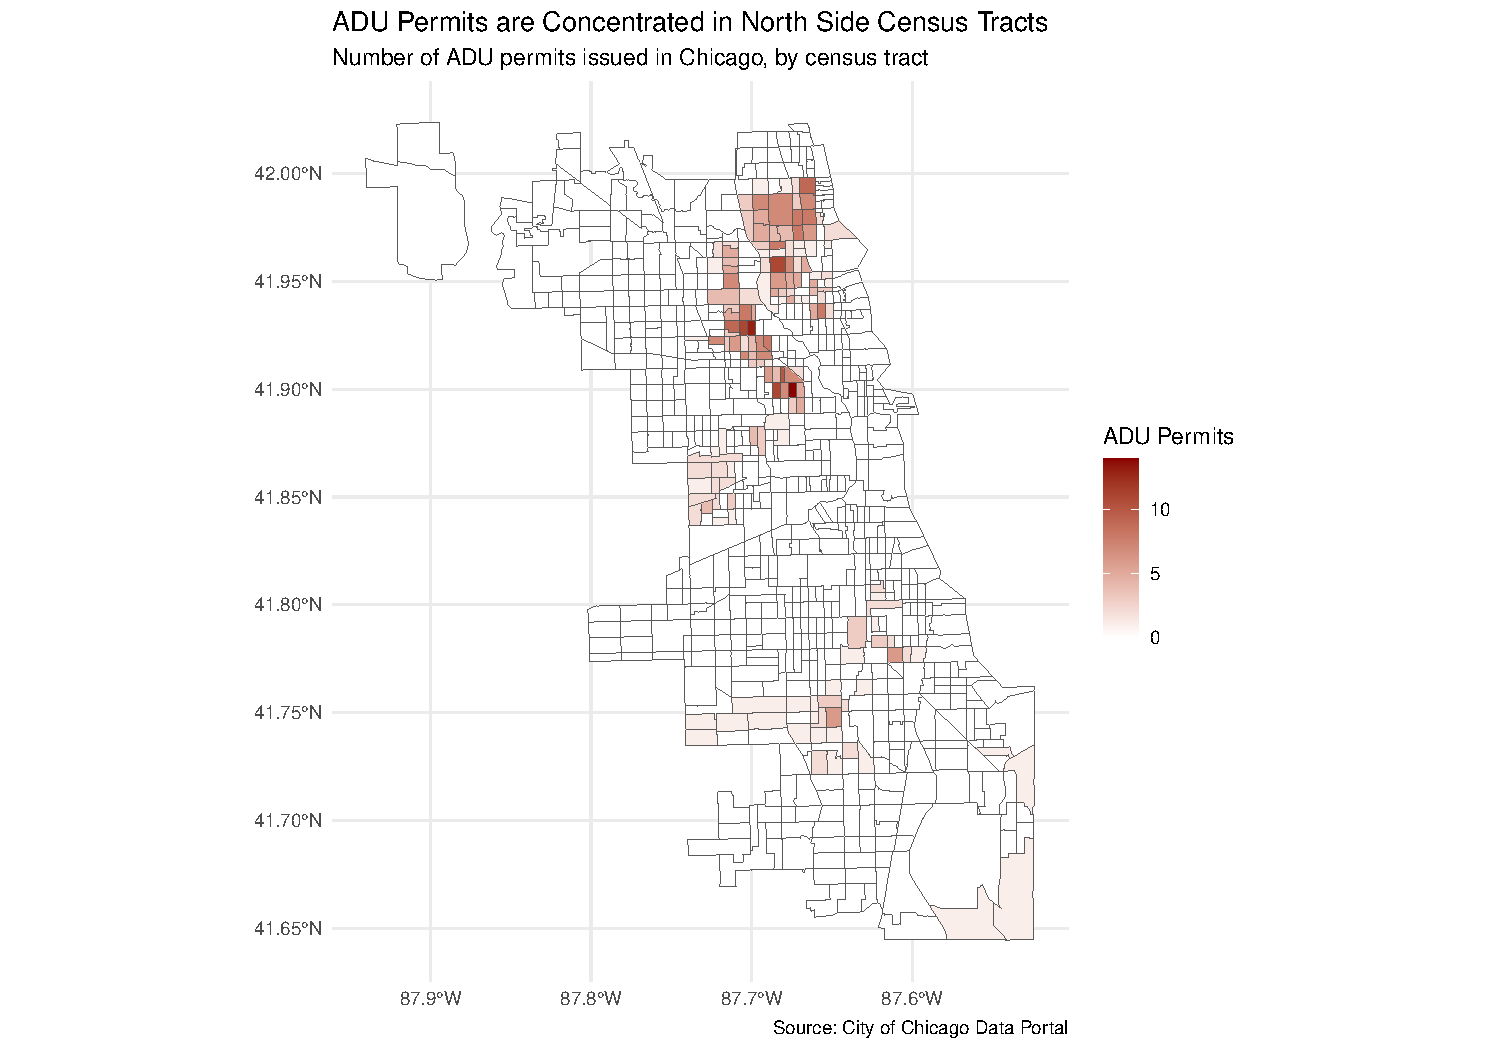
\includegraphics{Slides_files/figure-beamer/unnamed-chunk-2-1.pdf}
\end{frame}

\begin{frame}
\end{frame}

\end{document}
